\chapter{Experiments}

\section{Generating the obstacle forest (Poisson processes)}
\label{sec:Poisson-Process}

In order to generate the obstacle field for the experiments, which is to
resemble a forest, a spatial process called a \textit{Poisson process} is
employed. Poisson processes are used to model random configurations of points in
space'~\cite{kroeseSpatialProcessGeneration}, and hence are suitable for
generating a simulated forest. For the experiments below, a forest will be the
realization of a spatial Poisson process on \(\R^2\).

A few key parameters of the Poisson process has to be set for use in the
experiments below. Firstly, \(\lambda\) is the intensity of the spatial process.
For these experiments, the intensity will be held constant, and the process is
therefore homogeneous, as it does not vary with the position in space. One
interesting configuration could be to vary the intensity as the radius from
origo, and hence the difficulty in traversing the terrain would increase with
the distance travelled. However, the constant intensity setting was chosen to
keep things simple and uniform.

The algorithm for realizing a random Poisson measure~(\ref{def:Poisson-def}) is
taken from~\cite[Definition 1.1.1,p~34]{kroeseSpatialProcessGeneration}.

\begin{definition}[Generating a Poisson random measure]
  \label{def:Poisson-def}
  \begin{enumerate}
  \item Generate a Poisson random variable \(N ~ Poi(\mu(E))\).
  \item Draw \(X_1,X_2,\ldots,X_N ~ g\), where \(g(x) \lambda(x)/ \mu(E)\).
  \end{enumerate}
\end{definition}
where \(E\) is the set over which the points should be generated, and the
\textit{pdf} \(g(x_1, x_2) = \lambda(x)/\mu(E)\). Finally, \(\mu(E)\) is defined
as
\[
  \mu(E) = \int_{E} \lambda(x) dx.
\]

For the experiments the set \(E\) will be a square defined as
\[
  E = [-\alpha, \alpha]^2
\]
the density of the generated forest \(\lambda\) will be set to
\[
  \lambda = 0.09
\]
of which the resultant forest on a \(20 \times 20\) grid can be seen in
figure~(\ref{fig:poisson009})

\begin{figure}
  \centering
  \begin{minipage}[b]{0.4\textwidth}
    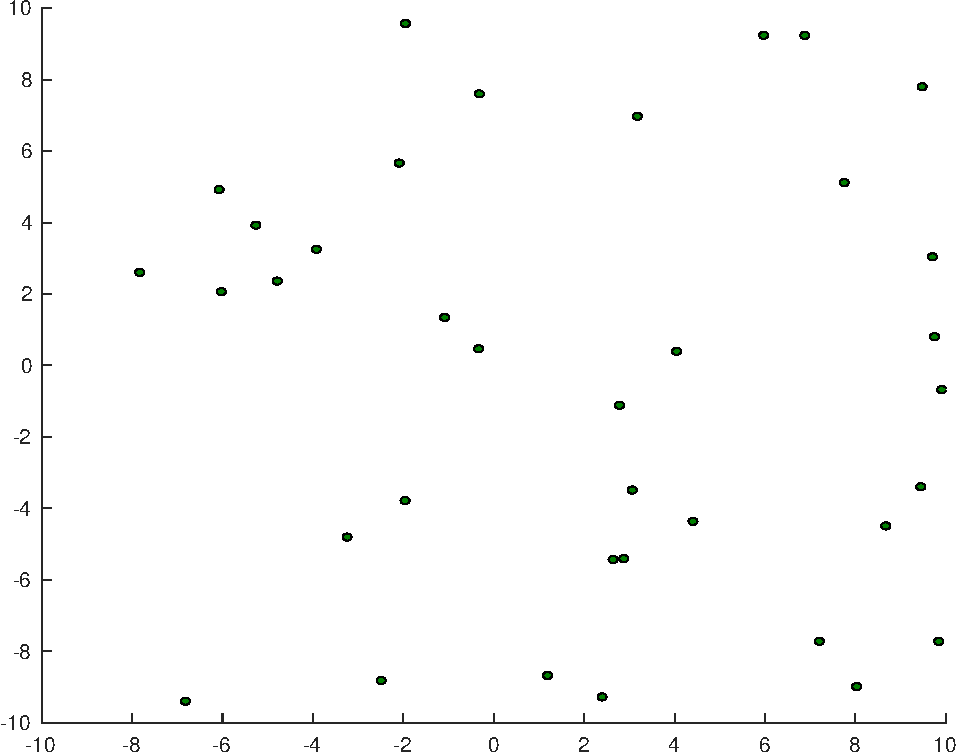
\includegraphics[width=\textwidth]{figures/experiments/poisson009}
    \caption{The resultant forest generated by a spatial Poisson process with
      intensity \(\lambda = 0.09\)}
    \label{fig:poisson009}
  \end{minipage}
  \begin{minipage}[b]{0.4\textwidth}
    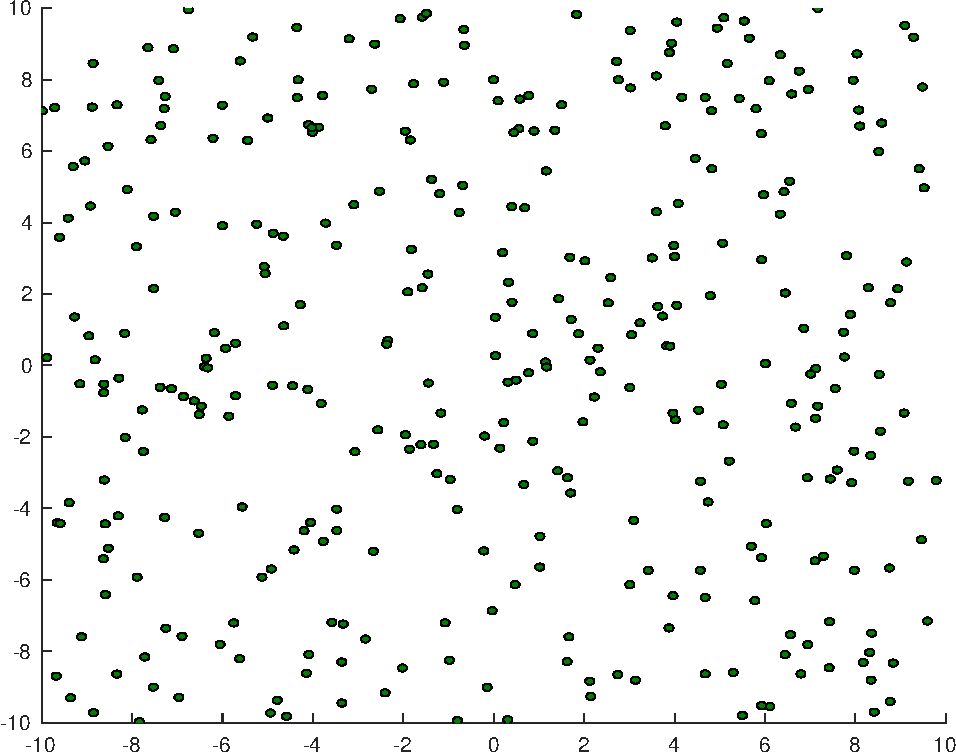
\includegraphics[width=\textwidth]{figures/experiments/poisson09}
    \caption{The resultant forest generated by a spatial Poisson process with
      intensity \(\lambda = 0.9\)}
    \label{fig:poisson09}
  \end{minipage}
\end{figure}

\section{Deciding upon the size of the vehicle and the obstacles}

The funnels generated thus far is created from a point model of the vehicle, and
it's dynamics. In the case that the grid that the simulations are run on are set
to have an increment of a meter, then the funnels from the basic set are given a
velocity of \([v(t)] = \si{m.s^{-1}}\), \([\theta] = \si{\radian\per\second}\),
and \([\dot{\theta}] = \si{\radian\per\second\per\second}\), where \([\cdot]\)
is the unit operator. The size of the vehicle is arbitrary, and can be chosen
freely, but if it is imagined as a radio controlled car, with a speed of
\(10\si{m.s^{-1}}\), then a size of \(30 \times 20 \si{\centi\metre} \) keeps
everything within the realm of a normal radio controlled car and its
capabilities. The mass is not relevant for our first order dynamics, but still
the vehicle is assigned a mass of \(1 \si{\kilo}\), so that the translation of
the model dynamics is not irrelevant.

\subsection{Expanding the size of the funnel by the size of the simulated
  vehicle}

The size of the vehicle in the original model a single point, and as such, not
accounted for in the funnel before running simulations. Therefore the funnels
have to be expanded in order for them to accomodate the necessary robustness
guarantees that are expected. However, the size of the vehicle only affects the
size of the funnel ellipsis projected down into the xy-plane. Therefore first
getting the projected size of the funnel where \(P \colon \R^4 \rightarrow
\R^2\) is a projection map with a projection matrix
\[
  P =
  \begin{bmatrix}
    I & \mathbf{0} \\
  \end{bmatrix}
\]
such that for the projected ellipsoid
\[
  \mathcal{E}_{p} = \set{\bar{x} \in \R^{2} \mid {\bar{x}}^{T}S_{k}^{(p)}\bar{x}
    \leq 1}
\]
and
\[
  S_{k}^{(p)} = \left( PS_{k}^{-1}P^T \right)^{-1}
\]
and \(\mathcal{E}_{p}\) is the projected set of the ellipsoid projected down
into the xy-plane~\cite{majumdarFunnelLibrariesRealtime2017}. In general an
ellipse centered at the origin is a linear transformation of the unit
circle~\cite{lay2005linear}. Exploiting this fact, expanding the radius of the
circle to encompass the vehicle model. Also taking into account that the matrix
\(S_{k}\) is \textit{Positive semidefinite}, and hence can be cholezky
factorized~\cite{lay2005linear}. The expanded ellipsis (which now contains all
the possible states of the vehicle model) is:

\begin{align*}
  S_{k}^{\mathcal{P}} &= R^{T}R \\
  \mathcal{C} &= \set{y \in \R^2 \mid y^{T}y \leq 1 + r_{vehicle}} \\
  S_{k}^{p'} &= R^{-1}y \\
\end{align*}

where \(S_{k}^{'}\) is the ellipsoid which contains the volume of the vehicle
for all verfied states in the funnel.

\subsection{The initial motion primitive set}

The basis set of motion primitives should be small, yet cover enough of the
finer movements of the vehicle, so that the motion of the vehicle can be near
continuous when composed together. Thus in order to generate a 'dense' set of
motion primitives the algorithm~(\ref{alg:initial-motion-primitives-generation})
is employed to generate points along the arch of a circle with \(N\) different
radii.


\begin{algorithm}[H]
  \label{alg:initial-motion-primitives-generation}
  \caption{Generating the initial motion primitives (TODO) - update with the new
    primitives!}
  \DontPrintSemicolon \SetAlgoNoLine

  \KwIn{
    \(n\) - Number of points along the arch \\
    \(r_{0}\) - Initial radius \\
    \(r_{f}\) - Final radius \\
    \(s\) - Stepsize (\(r_{n+1} = r_{n} + s\)) } \KwOut{\(\mathbf{X}\) -
    Endpoints matrix for the trajectory generator}

  \(\theta_{0} = \pi\) \;

  \For{\(r_{k+1} = r_{k} + s\)}{ \(\theta_{j} = \frac{\theta{0}}{2r}\) \;
    \(\theta_{stepsize} = \frac{\theta{j}}{(n-1)/2}\) \; \(\mathbf{X} \leftarrow
    (r_{k+1}, \theta=0)\) \; \For{\(i = 1 \) \KwTo \(\frac{n-1}{2}\)}{
      \(\theta_{ki} = i*\theta_{stepsize}\) \; \(\mathbf{X} \leftarrow (r, \pm
      \theta_{ki})\) \; }\; }\;
\end{algorithm}

The initial trajectories employed in the experiments can be seen in
figure~(\ref{fig:intial-trajectories-exp}), and the projected funnels overlaid a
sample in~(\ref{fig:sample-funnel-overlay}).

\begin{figure}
  \centering
  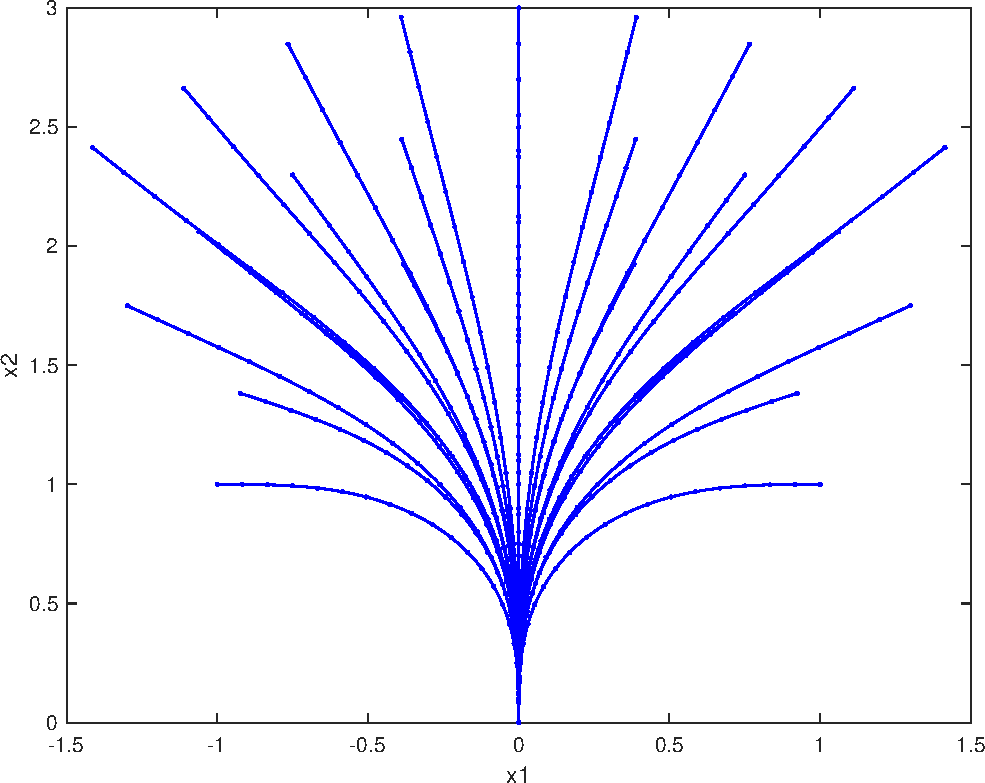
\includegraphics[scale=.5]{figures/experiments/initial-trajectories}
  \caption{The initial trajectories used in the \rrtfunnel{} algorithm.}
  \label{fig:intial-trajectories-exp}
\end{figure}

\begin{figure}
  \centering
  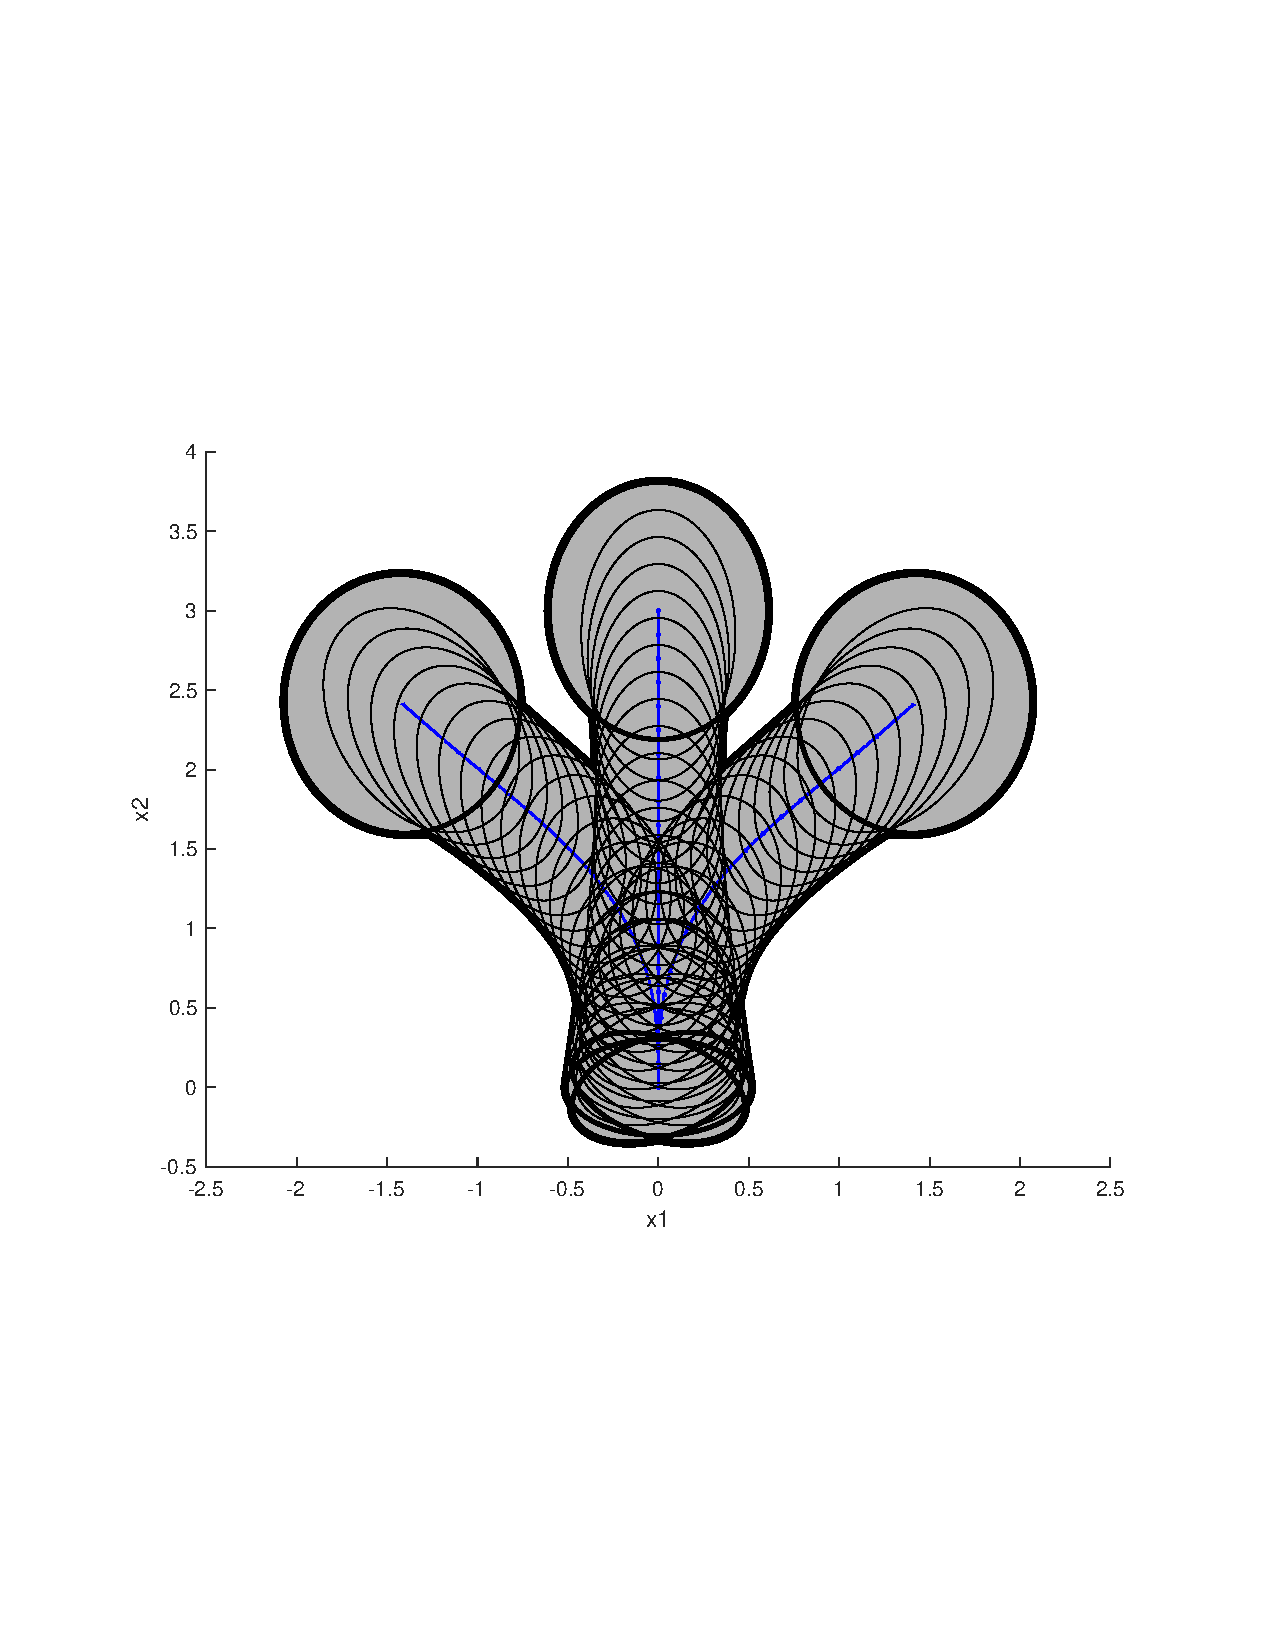
\includegraphics[scale=.5]{figures/experiments/sample-funnel-overlay}
  \caption{Three funnels from the initial trajectories with the projected
    funnels overlaid.}
  \label{fig:sample-funnel-overlay}
\end{figure}

\subsection{Sampling the goal set uniformly}

The goal set is a circle in the Euclidean plane, along with all possible goal
orientations for the vehicles heading, and the input. Hence, only the Euclidean
distance to the goal set is checked when running the algorithm, and \(\theta\)
and \(u\) are ignored. Sampling uniformly from a 

\subsection{Terrors of errors}

The funnel compuatations error out if too much uncertainty is added. In this
case that is velocity higher than two (which to be fair is a bit). Also, the
length of the funnels error out, meaning that funnels longer than approximately
.3 seconds, which is what they are now, will error out. Had there been more time
this should probably be resolved. A guess is that increasing the sampling
frequency, and/or increasing the initial size of the \(\rho\) guess would help.

From~\cite{tobenkinInvariantFunnelsTrajectories2010}, it is suggested that in
case a funnel is not verified using the \ac{SOS} programming method, one option
is to increase the size of \(\rho\) (the limiting factor on the size of the
funnel), and optionally increase the number of knot points (sampling points).

\subsection{What funnels are most oftenly(not a word) employed?}

Track and add some statistics on the most commonly employed funnels when testing
the algorithm.


\subsection{Experiments}

All three of the experiments will run with the motion primitive set pictured
in~(\ref{fig:intial-trajectories-exp}), with funnels surrounding them. Still all
three will have different uncertainty parameters.

The \rrtfunnel{} algorithm is benchmarked against the same algorithm, only the
funnels will not be surrounding the trajectories in the benchmark planner. Each
experiment will do a testrun of a hundred runs from

The end goal will not take pose into account, and will only be concerned with
getting within an \(\epsilon\) of the \((x,y)\) in the test map. For all the
experiments below, an \(\epsilon\) of 2\si{\metre} is given to the planners.

Each testrun will be run in a forest generated with the \textit{Poisson process}
method from~(\ref{sec:Poisson-Process}), and an intensity parameter (\(\lambda =
0.9\)), which should yield a pretty dense forest, and hence make collisions more
likely to happen.

The endgoal will be picked uniformly at random from the map, which is a 2D
Euclidean space (\ie \(\in (-\alpha,\alpha)\times(-\alpha,\alpha)\)), where
\(\alpha\) is the size of the map. The experiments will record the number of
collisions for each algorithm across all testruns, and the distance penalty
obtained total (which is the distance from the target, if the planner failed to
make it ther). The planners will run in the same environment at each test, with
the same initial seed, but the environments will be different from each run, as
the Poisson process generating the obstacle forest is random in nature. With
this test setup the difference between a planner which takes into account
uncertainty should become evident, and increasingly superior as more
uncertanties are added to the test environment.

Before the benchmark is run, all individual funnels in the base set are run with
a hundred simulations runs from random starting positions in its inlet, to check
if the invariant holds, and that the vehicle stays within the funnel at all
times. This, along with the check whether or not funnels are composable, as
in~(\ref{sec:composable-funnels}), then the invariant that the vehicle never leaves
multiple funnels composed holds.

Adding uncertainty to the testruns.

\(w = 2*wmax*rand - wmax\), in order to normalize around zero.

Below are the results from a hundred testruns across all the different test
parameters.

\subsubsection{Uncertainty in speed}

For the experiment

Model: (TODO) - syntax for the random variables -- choose one.
\begin{equation}
  \label{eq:model-dynamics}
  \mathbf{x} =
  \begin{bmatrix}
    x \\ y \\ \theta \\ \dot{\theta} \\
  \end{bmatrix}, \, \dot{\mathbf{x}} =
  \begin{bmatrix}
    -(v(t) + \randomSpeedVar{}) \sin(\theta) \\
    (v(t) + \randomSpeedVar{}) \cos(\theta) \\
    \dot{\theta} \\
    u \\
  \end{bmatrix}
\end{equation}

with \(\randomSpeedVar{}\) a random variable \(\randomSpeedVar{} \colon
\rightarrow [-2,2]\)

Uncertainties:
\begin{tabular}{ |c|c| }
  \hline
  \randomSpeedVar{} & 1 \\
  \hline
\end{tabular}

\subsubsection{Uncertainty in speed and input}
Model:
\begin{equation}
  \label{eq:model-dynamics}
  \mathbf{x} =
  \begin{bmatrix}
    x \\ y \\ \theta \\ \dot{\theta} \\
  \end{bmatrix}, \, \dot{\mathbf{x}} =
  \begin{bmatrix}
    -(v(t) + \randomSpeedVar{}) \sin(\theta) \\
    (v(t) + \randomSpeedVar{}) \cos(\theta) \\
    \dot{\theta} \\
    u \\
  \end{bmatrix}
  +
  \begin{bmatrix}
    0 \\
    0 \\
    0 \\
    \randomInputVar{} \\
  \end{bmatrix}
\end{equation}

Uncertainties:
\begin{tabular}{|c|c|}
  \hline
  \randomSpeedVar{} & 1 \\
  \randomInputVar{} & 5 \\
  \hline
\end{tabular}

\subsubsection{Uncertainty in speed, input and pos}

A nice combination of multiplicative and additive noise.

The model

\begin{equation}
  \label{eq:model-dynamics}
  \mathbf{x} =
  \begin{bmatrix}
    x \\ y \\ \theta \\ \dot{\theta} \\
  \end{bmatrix}, \, \dot{\mathbf{x}} =
  \begin{bmatrix}
    -v(t)\sin(\theta) \\
    v(t)\cos(\theta) \\
    \dot{\theta} \\
    u \\
  \end{bmatrix}
  +
  \begin{bmatrix}
    \randomPosXVar{}  \\
    \randomPosYVar{} \\
    \randomPosThetaVar{} \\
    \randomInputVar{} \\
  \end{bmatrix}
\end{equation}

Uncertainties:
\begin{tabular}{|c|c|}
  \hline
  \randomSpeedVar{} & 1 \\
  \randomPosXVar{} & 1\si{\centi\metre} \\
  \randomPosYVar{} & 1\si{\centi\metre}\\
  \randomPosThetaVar{} & 1 \\
  \randomInputVar{} & 5 \\
  \hline
\end{tabular}

TODO - maybe record a movie or two of the vehicle driving?

What happens if we add more uncertainty than what is modelled? - Run a simple
experiment, to check the robustness of both benchmark algorithms to unmodelled noise.